%\documentclass[border=10pt]{standalone}

\usetikzlibrary{decorations.text}
\usetikzlibrary{calc}
\usetikzlibrary{fit}
\usetikzlibrary{shapes}
\usetikzlibrary{arrows,positioning} 
\pgfmathsetmacro{\cubex}{4}
\pgfmathsetmacro{\cubey}{2}

\definecolor{light-gray}{gray}{0.80}

\tikzset{
    %Define standard arrow tip
    >=stealth',
    %Define style for boxes
    punkt/.style={
           rectangle,
           rounded corners,
           draw=black, very thick,
           text width=8em,
           minimum height=2em,
           
           text centered},
    % Define arrow style
    pil/.style={
           ->,
           very thick,
           %shorten <=2pt,
           shorten >=2pt,},
    sepLine/.style={
	dashed,
	very thick
    }
}


\tikzstyle{b} = [rectangle, draw, node distance=5cm, text 
width=9em, text centered, rounded corners, minimum height=4em, thick]
\tikzstyle{c} = [rectangle, draw, minimum height=15em, minimum width=10em, 
dashed]
\tikzstyle{l} = [draw,thick]

%\begin{document}
\begin{figure}[bh]
\begin{center}
\scalebox{1.0}{
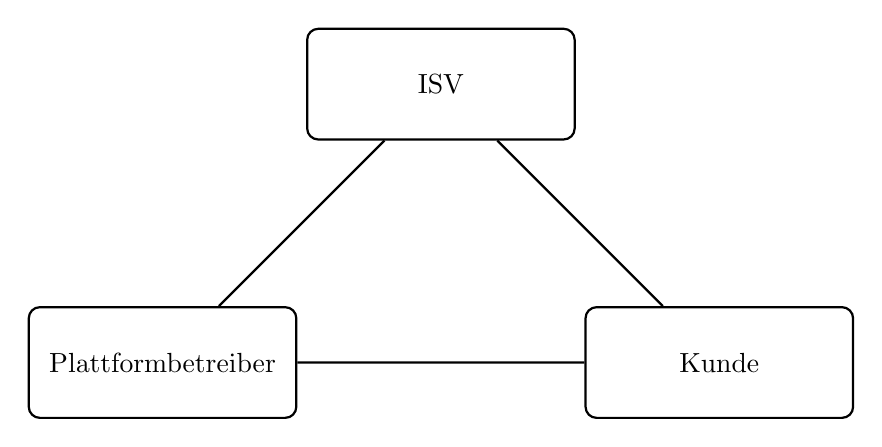
\begin{tikzpicture}[auto]
    \node[b] (ISV) {ISV};
    \node[b,below left of=ISV] (PAAS) {Plattformbetreiber};
    \node[b,below right of=ISV] (CLIENT) {Kunde};
    
    \path[l] (ISV) -- (PAAS) -- (CLIENT) -- (ISV);
    
 
\end{tikzpicture}
}
\caption{Das Beziehungsdreieck aus ISV, Plattformbetreiber und 
Kunde. Angelehnt an die Darstellung für SOAs 
aus \cite{changes_in_requirements_engineering}.}
\label{fig:cloud_oekosystem}
\end{center}
\end{figure}